\vspace{-0.3cm}

\section{Policy Evaluation}
\label{sec:experiments}
\label{sec:experiments:policy}
\vspace{-0.2cm}

Our policy evaluation tests whether representing interaction in a shared
metric space supports effective robot control. We examine task completion
across simulation benchmarks, robustness when observations and initial
states change, and execution on real-world robots.

\vspace{-0.2cm}

\subsection{Experimental Setup}
\label{sec:experiments:setup}
\vspace{-0.2cm}

\noindent\textbf{Training settings.}
We initialize the vision-language backbone from
Florence-2~\citep{xiao2023florence2} and randomly initialize all remaining
components. We consider two training settings: (1) \emph{with pretraining},
\method{} is pretrained on a mixture of real-robot, simulation, and
human hand demonstrations, then fine-tuned on each downstream benchmark
or dataset; (2) \emph{without pretraining}, \method{} (w/o Pretrain) is
fine-tuned directly on each target benchmark or dataset without the
mixed-dataset pretraining stage. More detailed training configurations
are provided in the appendix.

\noindent\textbf{Baselines.}
We compare against VLA policies
\citep{zheng2025xvla,sun2026vlajepa,black2024pizero,physicalintelligence2025pi05,abotm0},
video-based WAMs \citep{cosmospolicy,genieenvisioner,bi2025motus,li2026lingbotva,yuan2026fastwam}, and
3D-aware policies
\citep{qu2025spatialvla,wang2026lamp,guo2026xwam,zhou2026dexbev}.


\vspace{-0.2cm}

\subsection{Simulation Benchmarks}
\label{sec:experiments:simulation}
\vspace{-0.2cm}


\begin{table}[!b]
    \centering
    \small
    \setlength{\tabcolsep}{2.5pt}
    \renewcommand{\arraystretch}{0.93}
    \vspace{-0.5cm}
    \caption{Policy performance (\%, $\uparrow$). Our 1.7B model is evaluated
    with and without mixed-dataset pretraining. Bold and underlined scores
    denote the best and second-best results, respectively.
    LIBERO-Plus ranks use one-decimal precision.
    Dashes denote unavailable results.}
    \label{tab:experiments:simulation}
    \begin{adjustbox}{max width=0.94\linewidth}
    \begin{tabular}{@{}l*{12}{c}@{}}
        \toprule
        \multirow{2}{*}{Method}
        & \multirow{2}{*}{\shortstack{Params\\(B)}}
        & \multicolumn{5}{c}{LIBERO} & LIBERO-Plus
        & \multicolumn{2}{c}{RoboTwin 2.0} & \multicolumn{3}{c}{VLABench} \\
        \cmidrule(lr){3-7}\cmidrule(lr){9-10}\cmidrule(lr){11-13}
        & & Spatial & Object & Goal & 10 & Avg. & Overall & Clean & Rand. & SR & PS & IS \\
        \midrule
        \multicolumn{13}{l}{\textit{VLA Policies}} \\
        X-VLA & 1.0 & 98.2 & 98.6 & 97.8 & 97.6 & 98.1 & 71.4 & 72.88 & 72.84 & 29.4 & 51.2 & \underline{70.2} \\
        VLA-JEPA & 2.0 & 96.2 & 99.6 & 97.2 & 95.8 & 97.2 & 77.9 & -- & -- & -- & -- & -- \\
        $\pi_0$ & 3.0 & 96.8 & 98.8 & 95.8 & 85.2 & 94.15 & 53.6 & 65.92 & 58.40 & 29.4 & 44.1 & 55.0 \\
        $\pi_{0.5}$ & 3.0 & 98.8 & 98.2 & 98.0 & 92.4 & 96.9 & 85.7 & 82.74 & 76.76 & 48.1 & 62.3 & 64.9 \\
        ABot-M0 & 4.0 & 98.8 & \underline{99.8} & 99.0 & 96.6 & 98.6 & 80.5 & 80.42 & 81.16 & -- & -- & -- \\
        \midrule
        \multicolumn{13}{l}{\textit{Video-Based WAMs}} \\
        Cosmos Policy & 2.0 & 98.1 & \textbf{100.0} & 98.2 & 97.6 & 98.5 & 82.2 & -- & -- & -- & -- & -- \\
        GE-Act & 2.2 & 98.2 & 97.6 & 95.8 & 94.4 & 96.5 & 80.3 & -- & -- & -- & -- & -- \\
        % GigaWorld-Policy & 5 & -- & -- & -- & -- & -- & -- & 87.0 & 85.0 & -- & -- & -- \\
        LingBot-VA & 5.3 & 98.5 & 99.6 & 97.2 & 98.5 & 98.5 & 69.5 & \underline{92.93} & 91.55 & -- & -- & -- \\
        Fast-WAM & 6.0 & 98.2 & \textbf{100.0} & 97.0 & 95.2 & 97.6 & 51.5 & 91.88 & \underline{91.78} & -- & -- & -- \\
        Motus & 8.0 & 96.8 & \underline{99.8} & 96.6 & 97.6 & 97.7 & -- & 88.66 & 87.02 & -- & -- & -- \\
        \midrule
        \multicolumn{13}{l}{\textit{3D-Aware Policies}} \\
        SpatialVLA & 3.5 & 88.2 & 89.9 & 78.6 & 55.5 & 78.1 & -- & -- & -- & -- & -- & -- \\
        LaMP & 5.0 & \underline{99.4} & \underline{99.8} & 97.4 & 96.7 & 98.3 & 79.3 & -- & -- & -- & -- & -- \\
        X-WAM & 6.7 & -- & -- & -- & -- & -- & -- & 89.8 & 90.7 & -- & -- & -- \\
        Dex-BEV & -- & 98.2 & 98.0 & 97.8 & 97.0 & 97.8 & -- & 76.0 & 42.0 & -- & -- & -- \\
        \midrule
        \method{} (w/o Pretrain) & 1.7 & \textbf{99.8} & \underline{99.8} & \underline{99.4} & \underline{99.0} & \underline{99.5} & \underline{86.5} & 91.08 & 90.74 & \underline{50.3} & \underline{64.3} & \textbf{71.2} \\
        \method{} & 1.7 & \textbf{99.8} & \textbf{100.0} & \textbf{100.0} & \textbf{99.4} & \textbf{99.8} & \textbf{89.1} & \textbf{92.94} & \textbf{93.04} & \textbf{56.2} & \textbf{67.6} & 69.3 \\
        \bottomrule
    \end{tabular}
    \end{adjustbox}
    \vspace{-0.15cm}
\end{table}

We evaluate \method{} on single-arm and bimanual manipulation benchmarks.
LIBERO~\citep{liu2023libero} includes Spatial, Object, Goal, and
long-horizon LIBERO-10 suites; RoboTwin 2.0~\citep{chen2025robotwin}
covers 50 bimanual tasks under Clean and Randomized conditions.
VLABench~\citep{zhang2024vlabench} tests object and instruction
generalization across five tracks, measured by success rate (SR),
progress score (PS), and intention score (IS).
LIBERO-Plus~\citep{fei2025liberoplus} evaluates robustness to seven
types of observation, instruction, and initial-state perturbations.
Detailed protocols and per-task results are provided in the appendix.



\noindent\textbf{Manipulation performance.}
Tab.~\ref{tab:experiments:simulation} reports policy performance across
the evaluated simulation benchmarks. On LIBERO, \method{} achieves a
state-of-the-art average success rate of 99.8\%, with strong results
on spatial and long-horizon tasks. Without mixed-dataset pretraining,
it achieves 99.5\%, also exceeding all baselines.
On RoboTwin 2.0, \method{} achieves 92.94\% and 93.04\% under Clean
and Randomized conditions, respectively. Its 1.7B model outperforms
the compared methods while using fewer parameters than Fast-WAM (6B)
and Motus (8B). On VLABench, it achieves 56.2\% SR compared with
48.1\% for $\pi_{0.5}$, alongside a higher progress score.

\noindent\textbf{Robustness to distribution shifts.}
As shown in Tab.~\ref{tab:experiments:simulation}, \method{}
achieves the highest overall success rate of 89.1\%
on LIBERO-Plus. Appendix~\ref{app:libero_plus} reports the perturbation-wise results.
Under camera perturbations, it achieves 82.1\%, compared with 75.8\%
for Cosmos Policy and 64.5\% for LaMP. Both training settings show
strong viewpoint robustness, consistent with world-coordinate grounding
of visual observations.

Mixed-dataset pretraining improves overall success by 2.6 percentage points, with the largest gains under robot initial-state changes from 84.8\% to 94.2\%, and language perturbations from 77.6\% to 85.0\%. These improvements suggest better generalization to changes in both physical configuration and instruction phrasing.
As illustrated in Fig.~\ref{fig:experiments:mixed_dataset_training},
adding other data sources while keeping the number of RoboTwin samples per batch unchanged yields lower RoboTwin test XYZ error.
Together, these results support positive cross-dataset transfer
under our unified modeling formulation.

\vspace{-0.2cm}

\subsection{Real-world Evaluation}
\label{sec:experiments:real_world}
\vspace{-0.2cm}

We evaluate two real-world tasks: \emph{Organize Books} requires aligning
books with shelf compartments, while \emph{Pack the Ball} requires placing
a ball inside a bag and closing its zipper. We compare against $\pi_{0.5}$
and Fast-WAM using 20 trials per method per task.
As shown in Tab.~\ref{tab:experiments:real_world}, \method{} achieves
90\% and 80\% success on the two tasks, respectively, outperforming
both baselines.
Fig.~\ref{fig:experiments:real_world} shows representative executions.


\begin{table}[!t]
    \centering
    \newsavebox{\realworldimagebox}
    \sbox{\realworldimagebox}{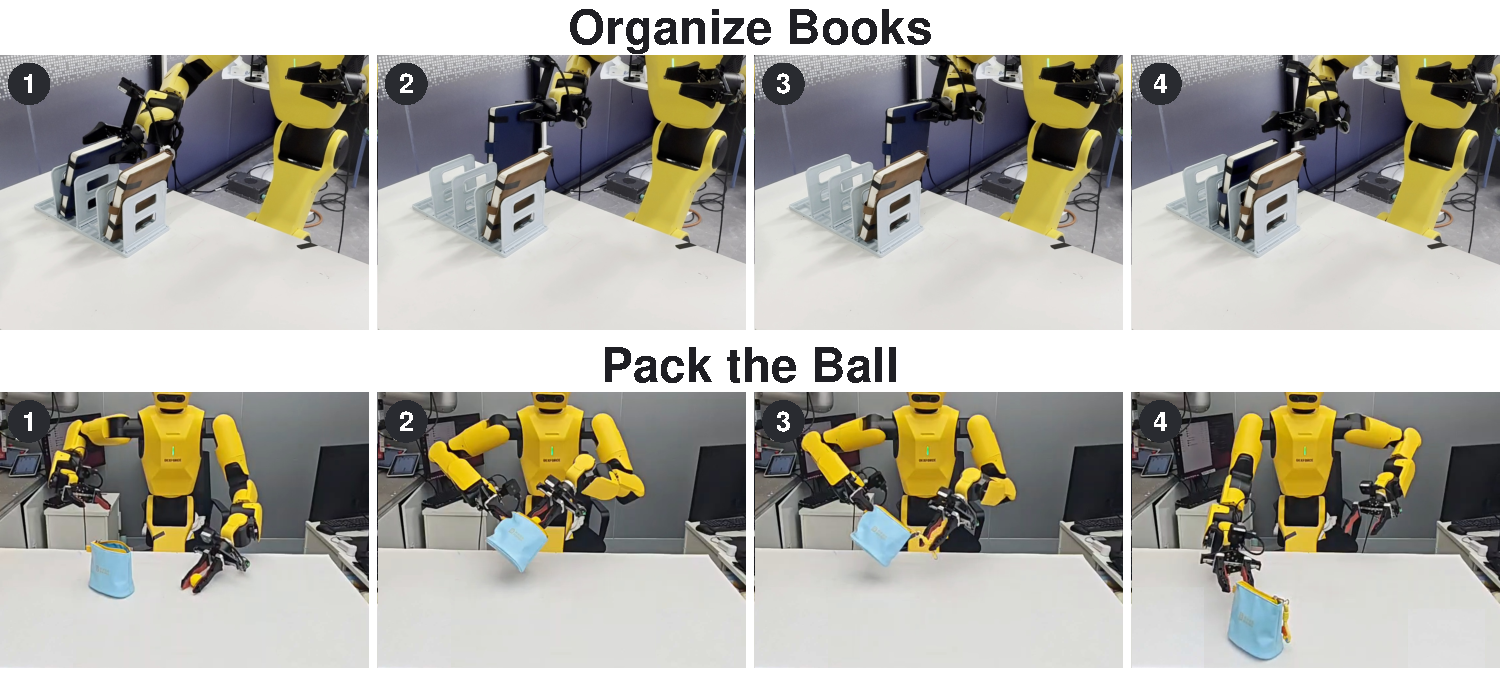
\includegraphics[width=0.65\linewidth]{figures/real_world_keyframes.pdf}}
    \begin{minipage}[t]{0.65\linewidth}
        \vspace{0pt}
        \usebox{\realworldimagebox}
        \makeatletter\def\@captype{figure}\makeatother
        \vspace{-0.9cm}
        \caption{Qualitative real-robot rollouts on \emph{Organize Books}
        and \emph{Pack the Ball}. Numbered keyframes show task progression
        through precise placement and sequential manipulation.}
        \label{fig:experiments:real_world}
    \end{minipage}\hfill
    \begin{minipage}[t]{0.33\linewidth}
        \vspace{0pt}
        \centering
        \makeatletter\def\@captype{table}\makeatother
        \setlength{\abovecaptionskip}{0pt}
        \caption{\raggedright Quantitative comparison results of real-robot experiments (20 trials per task).}
        \label{tab:experiments:real_world}
        \footnotesize
        % \setlength{\tabcolsep}{2pt}
        \setlength{\aboverulesep}{0pt}
        \setlength{\belowrulesep}{0pt}
        % \renewcommand{\arraystretch}{1.45}
        \renewcommand{\arraystretch}{1.0}
        \begin{tabular*}{\linewidth}{@{}l@{\extracolsep{\fill}}r@{}}
            \toprule
            \multicolumn{2}{@{}c@{}}{\colorbox[gray]{0.93}{\makebox[\dimexpr\linewidth-2\fboxsep\relax]{\strut\textbf{Organize Books}}}} \\
            \midrule
            $\pi_{0.5}$ & 15/20 (75\%) \\
            Fast-WAM & 13/20 (65\%) \\
            \method{} & \textbf{18/20 (90\%)} \\
            \midrule
            \multicolumn{2}{@{}c@{}}{\colorbox[gray]{0.93}{\makebox[\dimexpr\linewidth-2\fboxsep\relax]{\strut\textbf{Pack the Ball}}}} \\
            \midrule
            $\pi_{0.5}$ & 11/20 (55\%) \\
            Fast-WAM & 12/20 (60\%) \\
            \method{} & \textbf{16/20 (80\%)} \\
            \bottomrule
        \end{tabular*}
    \end{minipage}
    \vspace{-0.3cm}
\end{table}



\begin{table}[!b]
    \centering
    \small
    \setlength{\tabcolsep}{3pt}
    % \renewcommand{\arraystretch}{1.15}
    \renewcommand{\arraystretch}{0.96}
    \vspace{-0.85cm}

    \caption{LIBERO-Plus ablations without mixed-dataset pretraining.
    Checkmarks indicate enabled components.
    Success rates (\%) are reported for each perturbation;
    Overall pools all 10,030 evaluation episodes.}
    \label{tab:experiments:libero_plus_ablation}
    \begin{adjustbox}{max width=0.97\linewidth}
    \begin{tabular}{@{}cccc ccccccc c@{}}
        \toprule
        \multicolumn{4}{c}{Components}
        & \multicolumn{7}{c}{Perturbation Type}
        & Overall \\
        \cmidrule(lr){1-4}
        \cmidrule(lr){5-11}
        \shortstack{Visual\\3D PE}
        & \shortstack{Action-flow\\Loss}
        & \shortstack{History\\Tokens}
        & \shortstack{Scene-flow\\Loss}
        & Camera & Robot & Language & Light
        & Background & Noise & Layout & \\
        \midrule
        & & &
        & 50.47 & 59.48 & 67.14
        & 81.00 & 74.44 & 74.70
        & 71.80 & 67.58 \\

        & $\checkmark$ & $\checkmark$ &
        & 66.73 & 79.29 & 75.21
        & 94.57 & \underline{92.19} & 84.13
        & 84.46 & 81.35 \\

        $\checkmark$ & & $\checkmark$ &
        & 75.05 & 76.13 & 66.17
        & 90.72 & 87.45 & 86.45
        & 75.74 & 78.89 \\

        $\checkmark$ & $\checkmark$ & &
        & 69.04 & 64.71 & 72.41
        & 88.88 & 80.48 & 81.01
        & 79.80 & 75.92 \\

        $\checkmark$ & $\checkmark$ & $\checkmark$ &
        & \underline{79.11} & \underline{84.58} & \underline{77.10}
        & \underline{96.32} & \textbf{94.42} & \underline{89.07}
        & \underline{85.05} & \underline{85.74} \\

        $\checkmark$ & $\checkmark$ & $\checkmark$ & $\checkmark$
        & \textbf{81.86} & \textbf{84.84} & \textbf{77.62}
        & \textbf{96.67} & \textbf{94.42} & \textbf{89.82}
        & \textbf{85.11} & \textbf{86.47} \\
        \bottomrule
    \end{tabular}
    \end{adjustbox}
\end{table}



\vspace{-0.2cm}

\subsection{Ablation Study}
\label{sec:experiments:ablations}
\vspace{-0.2cm}

We ablate visual 3D positional encoding, action-flow supervision,
action-flow history tokens, and scene-flow supervision on LIBERO-Plus without
mixed-dataset pretraining.
As shown in Tab.~\ref{tab:experiments:libero_plus_ablation},
the first three ablations use a reference model without scene-flow
supervision, which achieves 85.74\% overall success.
Removing 3D positional encoding reduces success to 81.35\%,
with the largest drop under camera perturbations, from 79.11\%
to 66.73\%. This highlights the role of world-coordinate grounding
in relating visual observations to robot motion and improving
generalization across camera viewpoints.

Removing action-flow supervision reduces overall success to 78.89\%,
supporting the value of geometric motion supervision for action
learning.
Removing action-flow history tokens reduces overall success to 75.92\%,
with a drop of 19.87 percentage points under robot initial-state
perturbations, suggesting that recent motion provides useful context
beyond the current state.
Removing all three components yields a VLA-style baseline with
67.58\% success. Adding scene-flow supervision to the reference model improves overall
success from 85.74\% to 86.47\%, suggesting that future scene prediction
helps learn representations beneficial to action prediction, consistent
with findings in other WAMs~\citep{yuan2026fastwam}.


\vspace{-0.3cm}

\section{Action-Conditioned World Modeling}
\label{sec:experiments:world_model}
\vspace{-0.2cm}

\noindent\textbf{Evaluation setup.}
We evaluate action-conditioned scene prediction on held-out RoboTwin
rollouts using matched initial observations and robot-motion conditions,
with simulator states providing ground-truth point trajectories.
We compare against PointWorld~\citep{huang2026pointworld}, which directly
predicts 3D trajectories, and video-based Ctrl-World~\citep{ctrlworld}
and X-WAM~\citep{guo2026xwam}. Video predictions are lifted to 3D using
SpatialTrackerV2~\citep{xiao2025spatialtrackerv2}, with
Depth Anything 3~\citep{lin2025depthanything3} for Ctrl-World and native
depth predictions for X-WAM. Both are calibrated using only initial-frame
ground-truth depth.
We report Moving ADE and FDE for trajectory and endpoint accuracy,
Static ADE for background drift, and Moving Acc@1cm for the fraction
of moving-point predictions within 1\,cm of ground truth.
Detailed evaluation protocols are provided in Appendix~\ref{app:matched_action}.

\begin{figure}[!t]
    \centering
    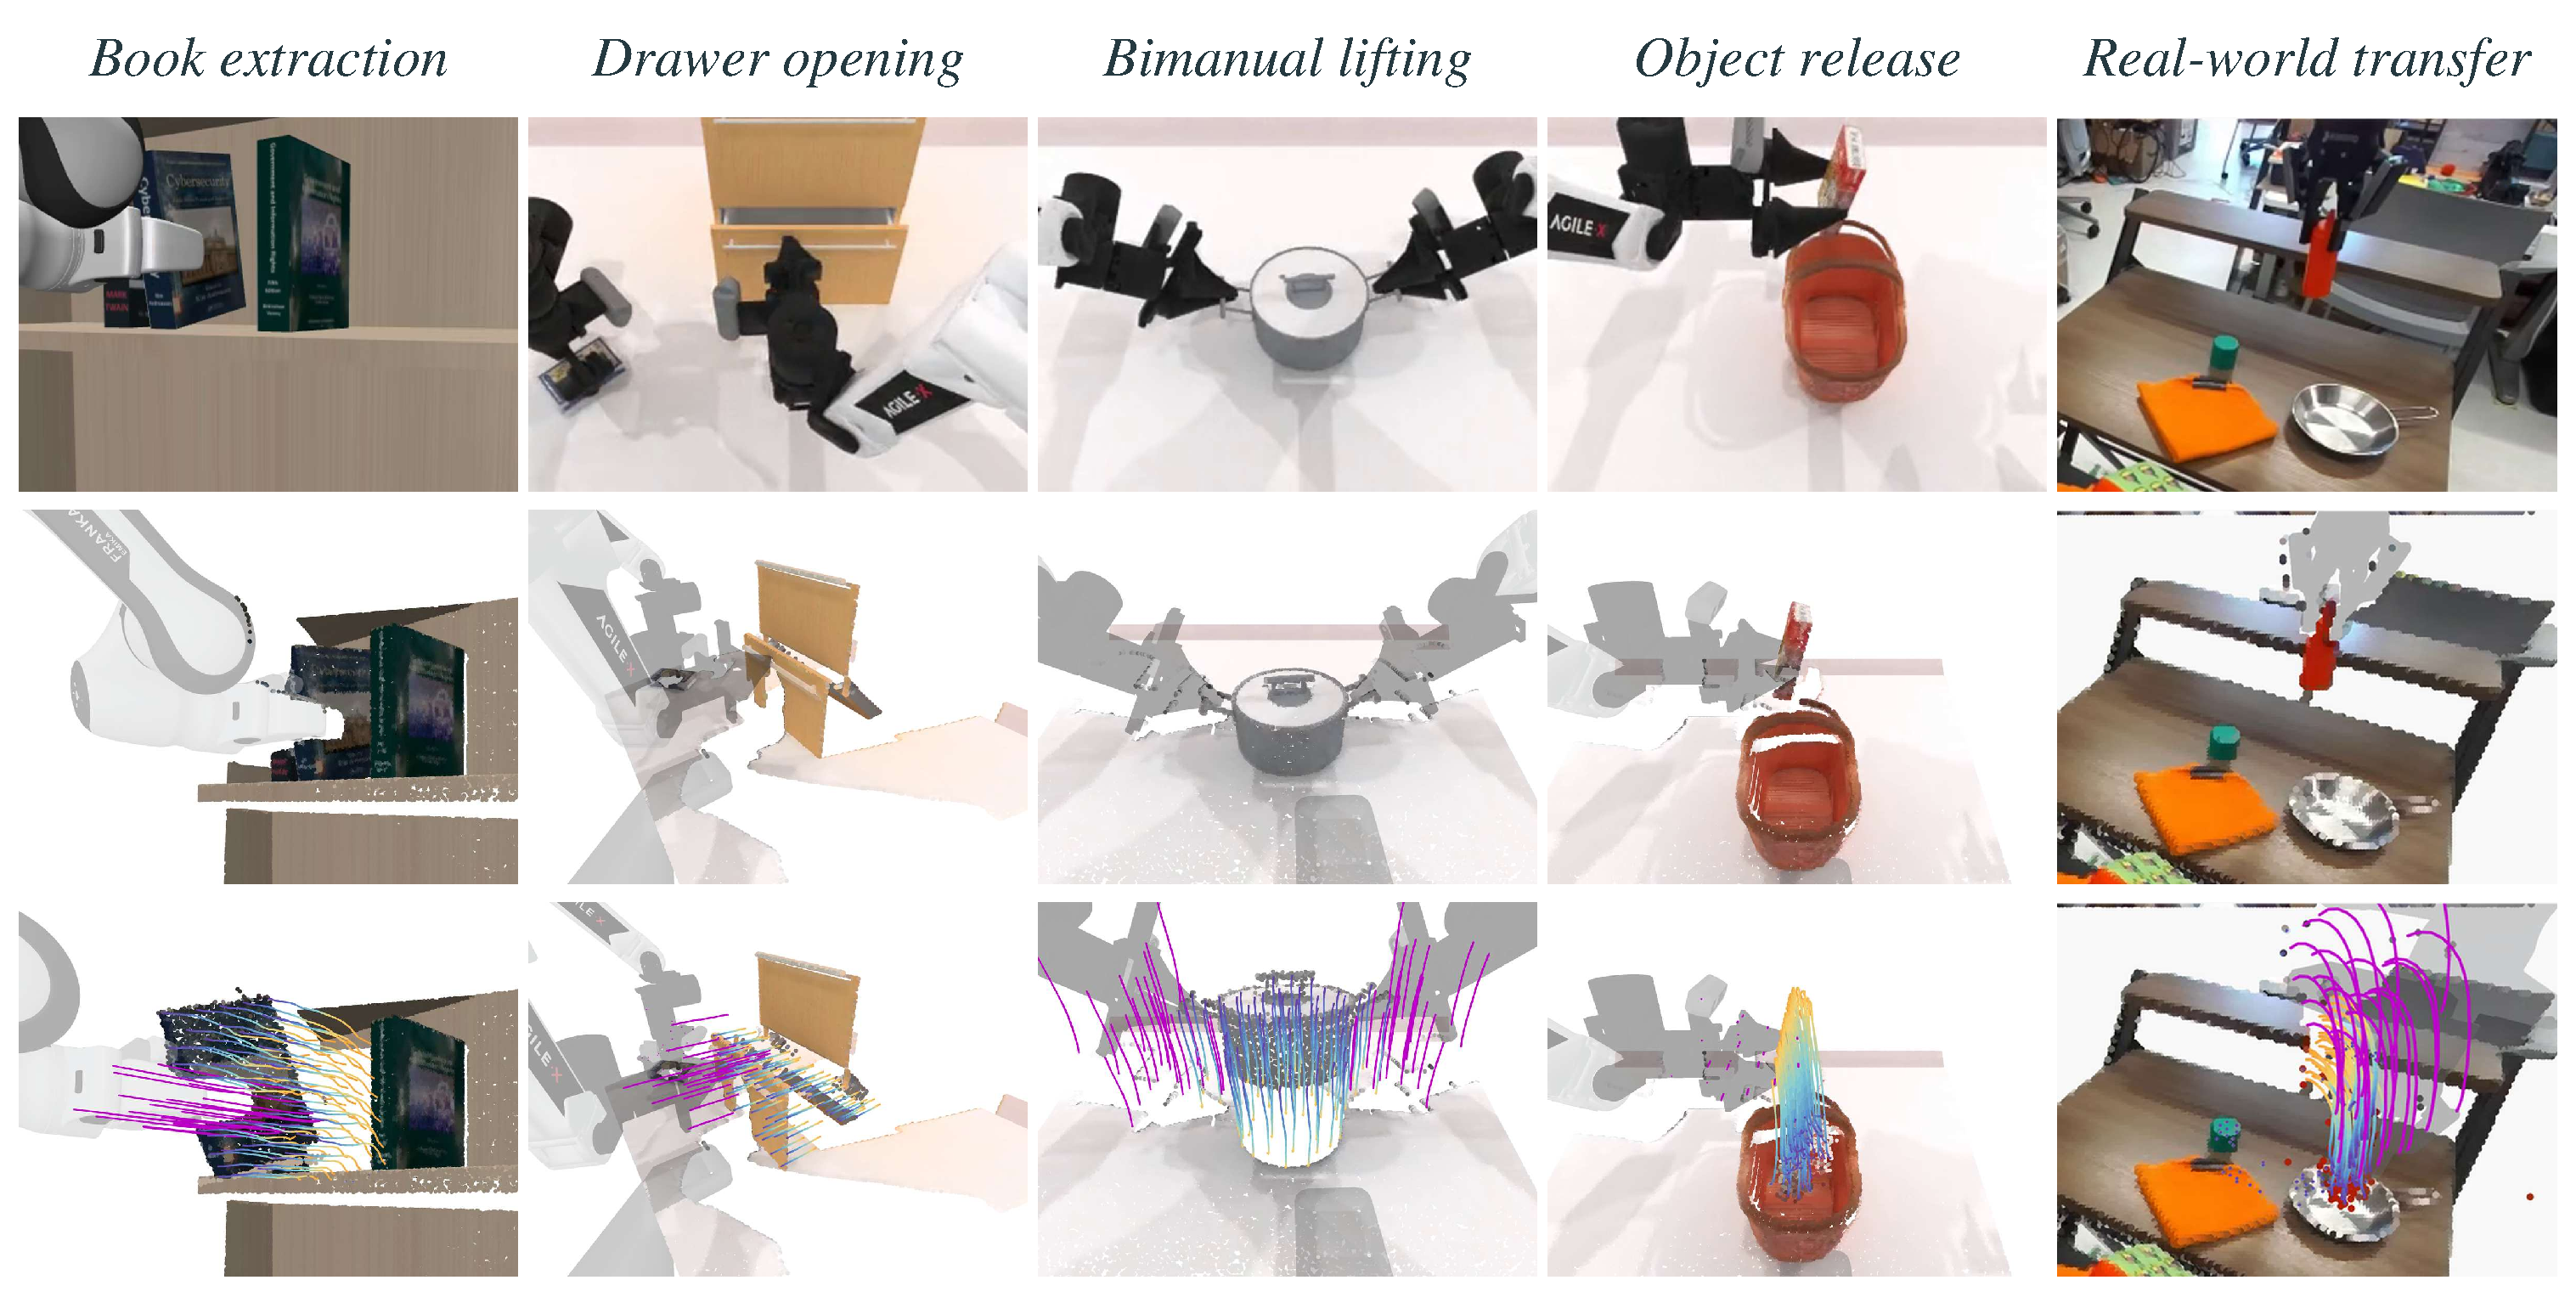
\includegraphics[width=0.9\linewidth]{figures/scene_flow_qualitative.pdf}
    \vspace{-0.5cm}

    \caption{\textbf{Action-conditioned scene-flow predictions.}
    Top: observed RGB images. Middle: initial point clouds.
    Bottom: predicted endpoint point clouds and scene trajectories
    (color gradient), conditioned on recorded gripper trajectories
    (purple). Translucent robot meshes indicate the corresponding poses.}
    \label{fig:experiments:scene_flow_qualitative}
    \vspace{-0.5cm}
\end{figure}

\begin{table}[!htbp]
    \centering
    \small
    \setlength{\tabcolsep}{4pt}
    % \renewcommand{\arraystretch}{1.10}
    \renewcommand{\arraystretch}{1.00}
    \vspace{-0.5cm}
    \caption{Action-conditioned scene prediction on RoboTwin.
    Errors are in cm ($\downarrow$); Acc@1cm is in \% ($\uparrow$).
    DA3 and STv2 denote Depth Anything 3 and SpatialTrackerV2, respectively.}
    \label{tab:experiments:world_model}
    \begin{adjustbox}{max width=0.97\linewidth}
    \begin{tabular}{@{}lcccc@{}}
        \toprule
        Method & Moving ADE $\downarrow$
        & Static ADE $\downarrow$
        & Moving FDE $\downarrow$
        & Moving Acc@1cm $\uparrow$ \\
        \midrule
        PointWorld & \underline{0.656} & \underline{0.084}
        & \underline{1.050} & \underline{88.22} \\
        Ctrl-World + DA3 + STv2
        & 3.310 & 0.369 & 5.503 & 41.54 \\
        X-WAM + STv2
        & 2.286 & 0.122 & 3.886 & 49.69 \\
        \textbf{\method{}} & \textbf{0.427} & \textbf{0.043}
        & \textbf{0.825} & \textbf{92.31} \\
        \bottomrule
    \end{tabular}
    \end{adjustbox}
    \vspace{-0.3cm}
\end{table}

\noindent\textbf{Action-conditioned scene prediction.}
\method{} achieves the best results across all four metrics, as shown
in Tab.~\ref{tab:experiments:world_model}, reducing Moving ADE from
0.656 to 0.427\,cm relative to PointWorld while improving moving-point
accuracy and reducing static-region drift.
Fig.~\ref{fig:experiments:scene_flow_qualitative} illustrates object
motion and resulting spatial configurations conditioned on gripper
trajectories. The simulation examples use training clips and DROID
example shows real-world scene prediction without real-world
scene-flow supervision.

\noindent\textbf{Action-scene consistency.}
We test whether predicted scene changes agree with the consequences of
the model's own actions on three RoboTwin tasks. \method{} achieves the
best consistency between predicted scene evolution and executed actions
among the compared WAMs. Appendix~\ref{app:future_action_alignment}
provides the evaluation details and full results.
